\section{Розробка алгоритму}
Для побудови прогностичних моделей розроблено та використовується величезна кількість алгоритмів. В загальному вигляді процес використання прогностичних моделей для вхідних даних можна представити у вигляді діаграми на рис. \ref{fig:data_process}.

\begin{figure}[h!]
  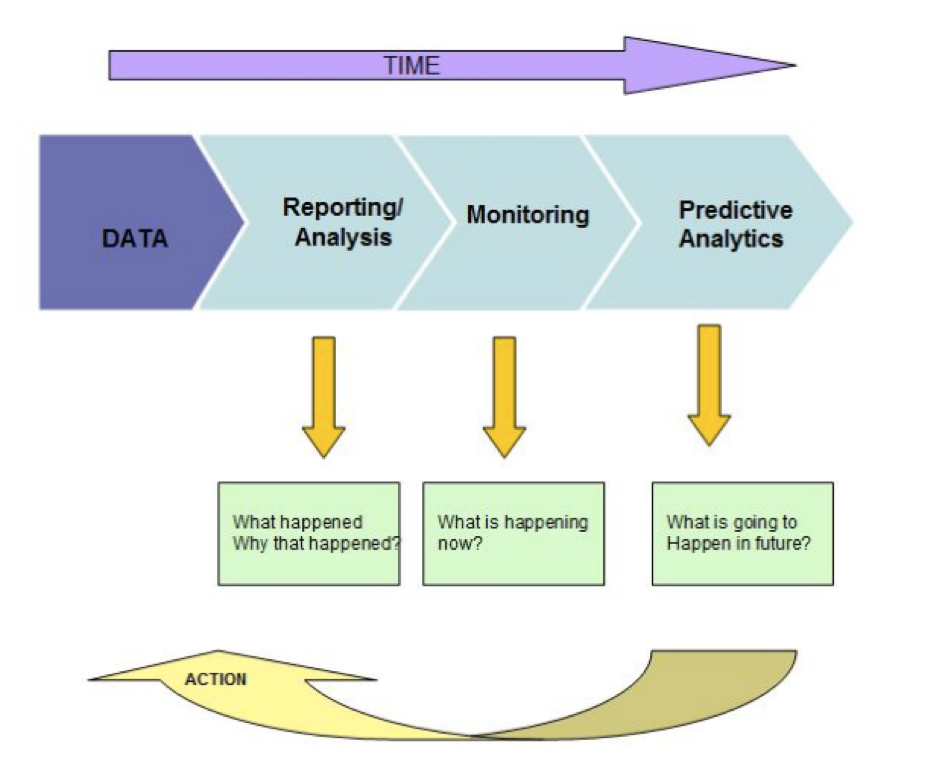
\includegraphics[width=\linewidth]{figures/data_process.png}
  \caption{Процес зміни даних з часом}
  \label{fig:data_process}
\end{figure}

!HEREDOC

\subsection{Оптимізація алгоритмів для використання у предметній галузі}
Оскільки велика кількість алгоритмів вимагають специфічного середовища чи платформи, а для побудови інших необхідні значні обчислювальні потужності, постає проблема платформозалежності та неможливості використання кращих підходів за умови існування додаткових обмежень. Щоб уникнути даних проблем, достатньо розробити рішення, що буде відповідати поставленим нижче вимогам:
\begin{itemize}  
	\item доступ користувача до коду моделі на будь-якій платформонезалежній мові, що дозволить запускати її в довільному середовищі та не спиратися на використання сторонніх бібліотек;
	\item будова моделі та деталі її внутрішньої реалізації повинні бути відкритими, тобто користувач повинен мати змогу переглянути вихідний код і в разі необхідності самостійно відтворити довільний крок та отримати аналогічний результат передбачення для однакового набору вхідних даних;
	\item модель повинна мати точність максимально наближену до точності моделей, що показують найкращі результати для вибраних вхідних даних. Модель повинна мати аналогічні показники щонайменше для 95\% всіх вхідних наборів даних;
	\item виконання коду програми повинно бути швидким (близько 1 мс на рядок вхідних даних).
\end{itemize}

Єдиного рішення, що дозволило б відмовитися від наявних алгоритмів на користь одного, визначеного вимогами вище, поки що немає, але існує підхід, що дозволяє покрити перелік всіх умов. Даний підхід носить назву апроксимаційної моделі [1]. Основна ідея полягає в припущенні, що деяка відносно проста модель, побудована на основі передбачень більш складної моделі може показати схожі результати в межах допустимого відхилення. Саме такою моделлю є RuleFit-модель [2], або модель на основі класу визначених правил. Принцип роботи полягає в серії тренувань дерев вибору на вхідних даних з наступною конвертацією гілок дерев в класи правил. Наприклад, одне правило може виражатися такою формулою: $20 < age <= 30 and income > 10000$. Новий набір даних створюється на основі оригінальних вхідних даних, генеруючи набір індикаторів $0/1$ таким чином, що кожен рядок позначає негативне чи позитивне значення в залежності від результату застосування правила до цього рядка. Дані індикатори потім використовуються в якості значень передбачення для узагальненої лінійної моделі.
\begin{equation}
    \label{eq:linear_model}
    y(w, x) = w_{0} + w_{1}x_{1} + \ldots + w_{p}x_{p}
\end{equation}

Формула \ref{eq:linear_model} описує звичайну модель, що є лінійною комбінацією вхідних значень та вектора коефіцієнтів $w$, а  $y$ – це значення, для якого здійснюється передбачення.

RuleFit є простою моделлю в тому плані, що це лише список правил з відповідними коефіцієнтами для кожного з них. Однак існують і недоліки, пов'язані з тим, що класи правил можуть містити подібні правила, що ускладнює інтуїтивне розуміння впливу коефіцієнтів, тобто вносить складність для розуміння людиною.

Існує дві основних частини в реалізації алгоритму: безпосереднє тренування і передбачення та rulefit задача. Дана задача містить багато параметрів, найголовнішим з яких є альфа-параметр, що визначає розмір регуляризації [3], що застосовується до лінійної моделі RuleFit.

Кінцевим етапом стоврення такої моделі повинна бути валідація згенерованого коду. Оскільки немає жорсткої прив’язки до використовуваної мови, потрібно переконатися, що код компілюється та виконується коректно. Далі потрібно запустити код та зберегти файл з прогнозованими значеннями для подальшого порівняння зі значеннями, що отримуються від оригінальної моделі. Якщо похибка лежить в межах допустимого відхилення валідація вважається успішно пройденою.

